\chapter{Communication interfaces}
All the communication interfaces are available via dedicated connectors.

\begin{ZubaxTableWrapper}{Connectors types}
    \begin{ZubaxWrappedTable}{| X | X |}
    Connector name          & Connector type    \\
    CAN1 (2 connectors)     & JST BM04B-GHS     \\
    CAN2 (2 connectors)     & JST BM04B-GHS     \\
    AUX                     & JST BM04B-GHS     \\
    USB                     & micro B USB 2.0   \\
\end{ZubaxWrappedTable}
\end{ZubaxTableWrapper}


\begin{figure}[!hbt]
    \centering
    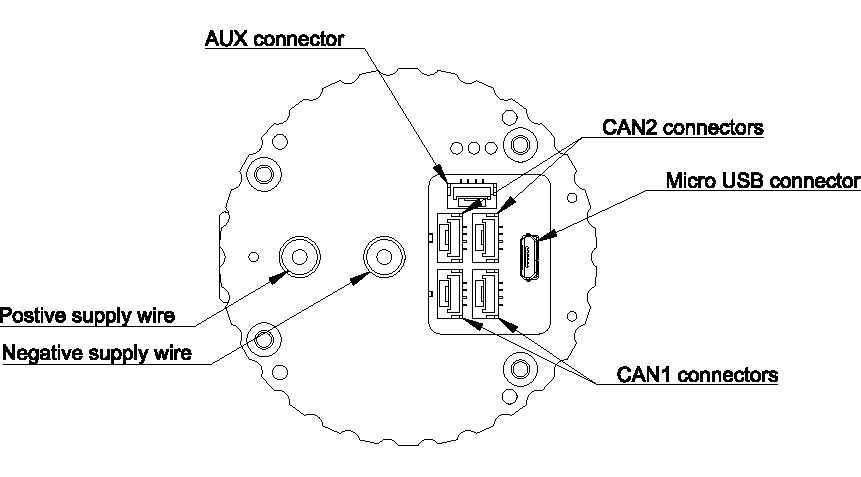
\includegraphics[width=1\textwidth]{figures/connectors_placement.pdf}
    \caption{Connectors drawing}
\end{figure}

\begin{figure}[!hbt]
    \centering
    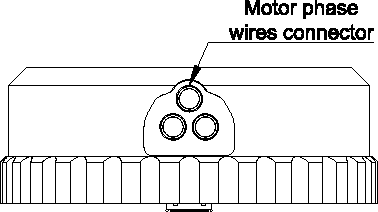
\includegraphics[width=0.5\textwidth]{figures/phase_wires.pdf}
    \caption{Motor phase wires connector drawing}
\end{figure}

\newpage

\section{CAN bus}
 The device is equipped with a doubly redundant ISO 11898-2 CAN 2.0A/B interface.
 Each CAN interface has two standard UAVCAN Micro connectors
 \footnote{Refer to \url{http://uavcan.org} for more information on UAVCAN.} 
 joined in parallel.  The device does not terminate the CAN bus internally.
 CAN2 (the secondary CAN bus interface) can only be used in configurations with redundant CAN bus.
 If the bus is not redundant, only CAN1 (the primary CAN bus interface) can be used.
 Connectors of the unused CAN bus interfaces should be left empty.

\begin{ZubaxSimpleTable}{CAN bus connectors pinout}{|c X X X[3]|}
	Pin no. & Type         & Name      & Comment \\
	1       & Power        & PWR       & Not connected to the device's circuits internally.\\
	2       & Input/Output & CAN H     & \\
	3       & Input/Output & CAN L     & \\
	4       & Ground       & GND       & \\
\end{ZubaxSimpleTable}

\subsection{BEC output}
Zubax Komar features software-controllable BEC outputs (1 per each CAN interface).
It is available on bus power supply pins of UAVCAN connectors.
BEC outputs are protected against short circuit,
maximum output current is 500 mA per CAN interface.
Outputs are also protected from the reverse current flow with ideal diodes.
BEC outputs for both CAN interfaces is controlled with a single software parameter.

\section{USB interface}
The device implements a full-speed USB 2.0 port with the standard CDC ACM interface 
(also known as \mbox{virtual serial port}). 
The device features driverless compatibility with all major operating systems (\mbox{Windows}, GNU/Linux, Mac OS).
The physical connector type is USB micro B (which is one of the most common device-side USB connector types). 
Zubax Komar will report the following properties to the USB host:

\begin{itemize}
\item Vendor ID -- 0x1D50
\item Product ID -- 0x60C7
\item Vendor string -- Zubax Robotics 
\item Device description string -- Zubax Robotics Telega
\end{itemize}

This interface uses Popcop protocol to communicate with Kucher(GUI software for \text{T\'elega} based products)

\section{GPIO}
Zubax Komar is equipped with 2 GPIO pins that are available on the AUX connector.
While GPIO2 can be used as GPIO only, GPIO1 has additional alternate functions that may be enabled in software:
\begin{itemize}
    \item RC PWM input
    \item Thermistor input
\end{itemize}

\begin{ZubaxSimpleTable}{AUX connector pinout}{|c X X X[3]|}
	Pin no. & Type         & Name      & Comment                        \\
	1       & Power        & PWR       & 5 V power line output          \\
	2       & Input/Output & GPIO1     & RC PWM input/Thermistor input  \\
	3       & Input/Output & GPIO2     &                                \\
	4       & Ground       & GND       &                                \\
\end{ZubaxSimpleTable}

\subsection{Thermistor input}
Zubax Myxa allows motor windings temperature measurement by means of PTC thermistor.
It supports the following thermistors: KTY84/130, KTY81/120, KTY83/120. No additional components are needed
to connect the thermistor. The thermistor model is selected in the firmware.
Thermistor should be connected between GPIO1 and GROUND pins of the AUX connector.
Most of the commercially available BLDC motors do not have any temperature sensor embedded and require
the installation of the sensor by the end user.

\subsection{RC PWM input}
Although RC PWM may be considered an outdated interface due to its analog nature that makes it both pretty slow
and prone to errors caused by electromagnetic interference, it is still probably the most widespread
ESC interface in the industry. Zubax Komar can support RC PWM input.
It should be connected to GPIO1 of AUX connector and then configured in firmware.
\text{T\'elega} firmware allows for a very flexible configuration of RC PWM interface.

For more detailed description please refer to \text{T\'elega} reference manual or
\href{https://forum.zubax.com/t/quick-start-guide-for-myxa-v0-1/911}{Myxa quick start guide}